\subsection{View Synthesis}\label{subsec:viewsynthesis}

View synthesis is a technique used to generate views between two input views.
Figures~\ref{fig:vs_left_input} and~\ref{fig:vs_right_input} give the two input images and their associated disparity
map (generated with~\citep{stereomatching}).
We implemented view synthesis with the assumption that the two camera positions differ only by a $x$-translation
($R=I,t=\left[x\hspace*{2mm} 0\hspace*{2mm} 0\right]^t $).

\begin{figure}[ht]
    \centering
    \captionsetup{justification=centering}
    \begin{minipage}{.5\textwidth}
        \centering
    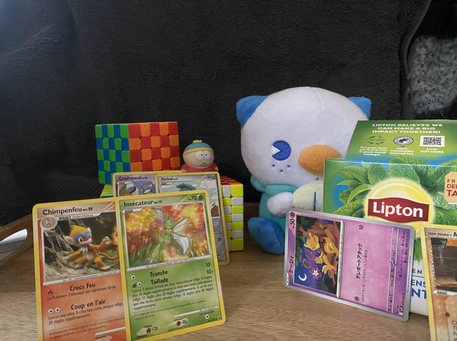
\includegraphics[width=0.7\textwidth]{assets/viewsynthesis/left_rect}
    \end{minipage}%
    \hfill
    \begin{minipage}{.5\textwidth}
        \centering
    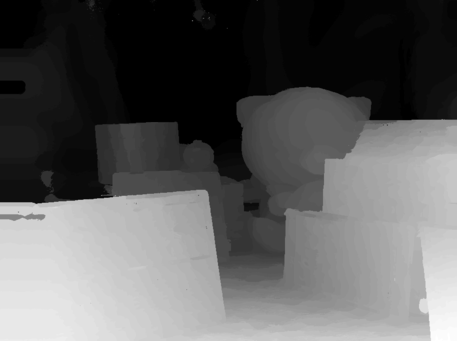
\includegraphics[width=0.7\textwidth]{assets/viewsynthesis/disparity_map_left}
    \end{minipage}
    \caption{The left input view with the associated disparity map.}
    \label{fig:vs_left_input}
\end{figure}

\begin{figure}[ht]
    \centering
    \captionsetup{justification=centering}
    \begin{minipage}{.5\textwidth}
        \centering
    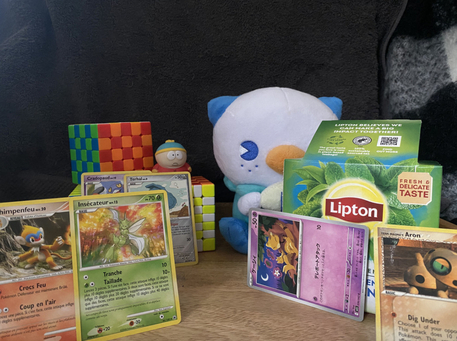
\includegraphics[width=0.7\textwidth]{assets/viewsynthesis/right_rect}
    \end{minipage}%
    \hfill
    \begin{minipage}{.5\textwidth}
        \centering
    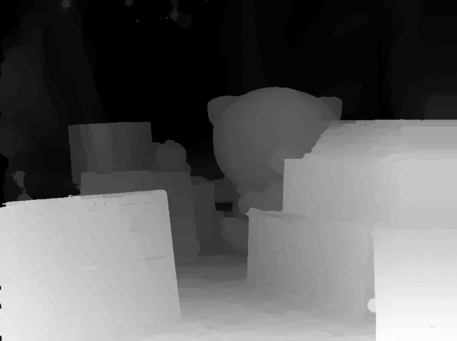
\includegraphics[width=0.7\textwidth]{assets/viewsynthesis/disparity_map_right}
    \end{minipage}
    \caption{The right input view with the associated disparity map.}
    \label{fig:vs_right_input}
\end{figure}

Given the two images and their respective disparity map, it is easy to build a new image that is located at the
point $0<\alpha<1$ between the two images ($\alpha=0$ corresponds to the left image, $\alpha=1$ corresponds to the
right image and $\alpha=1/2$ corresponds to the view exactly in the middle of the two shots).
For all pixels $(i,j)$ in the left image, we know that it would land at position $(i-\alpha d,j)$ for view $\alpha$ if
the disparity was $d$ ($d>0$).
Doing this for all pixels in the image, we get a barebones version of view $\alpha$.
If two pixels land on the same pixel in the output image, we keep the one with the highest disparity (since it's the
one with the smallest depth and therefore should appear in front of the other).
If this happens, we necessarily will have empty pixels in the output image.
Empty pixels can also appear because of disocclusions.
To fill in (not necessarily all) empty pixels, we can build another output image but this time using only the right
image as a base, where pixel $(i,j)$ is mapped to pixel $(i+\alpha d,j)$ in the output image.

The above method is known as forwards view synthesis.

It could still be the case that some pixels are left empty by this method.
In this case, we can use backwards view synthesis.
The idea of this method is, instead of projecting the pixels into the output image, look for every pixel in the output
image which pixel lands the closest.
We again do this process from left to right and from right to left.
Merging the two images is not as trivial as before since all pixels are filled: we cannot simply discard the pixel that
is empty, we always have two candidates.
To solve this issue, we can attribute a score to each pixel in the two generated images and keep the pixel with the
better score.
The score is the distance between the pixel and the position where the pixel that was mapped to it fell.
That is, if there is a pixel at position $(i,j)$ in the output image that came from a pixel $(i',j)$ with disparity $d$,
the score for $(i,j)$ is $|i-(i'+\alpha d)|$.

The code that handles forwards and backwards view synthesis can be found in function the \texttt{render\_one} of
\texttt{view\_synthesis/src/view\_synthesizer/ViewSynthesizer.py} (\textit{QV.1}).

To apply everything on our test images, we had to take pictures of a scene while being careful to only move the camera
in the $x$-axis.
We achieved this using a ruler and a lego rail.
The images were then corrected for radial distortion and rectified
(since it is virtually impossible to get a true $x$-translation of the camera).
The two disparity maps were obtained using the IPOL paper~\citep*{stereomatching} (after tweaking the parameters).
The images were then cropped to remove the empty pixels that came from the rectification.
Finally, the disparity maps were cleaned by hand, to finally obtain the result of figure~\ref{fig:vs_cleaned_disp}
(there were visible artifacts as well as blatantly wrong disparities for certains regions of the images
as we can see in figure~\ref{fig:vs_left_input} and~\ref{fig:vs_right_input}).

\begin{figure}[ht]
    \centering
    \captionsetup{justification=centering}
    \begin{minipage}{.5\textwidth}
        \centering
    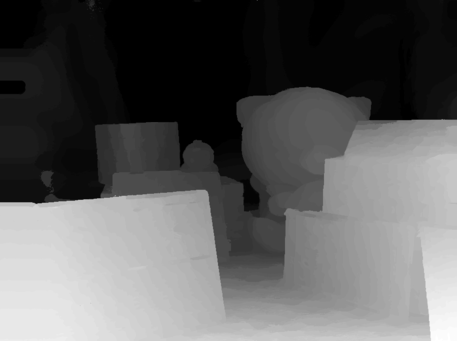
\includegraphics[width=0.7\textwidth]{assets/viewsynthesis/disparity_map_left_clean}
    \end{minipage}%
    \hfill
    \begin{minipage}{.5\textwidth}
        \centering
    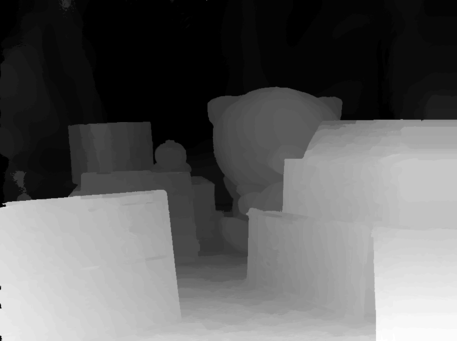
\includegraphics[width=0.7\textwidth]{assets/viewsynthesis/disparity_map_right_clean}
    \end{minipage}
    \caption{The cleaned-up disparity maps.}
    \label{fig:vs_cleaned_disp}
\end{figure}

\begin{figure}[ht]
    \centering
    \captionsetup{justification=centering}
    \begin{minipage}{.5\textwidth}
        \centering
    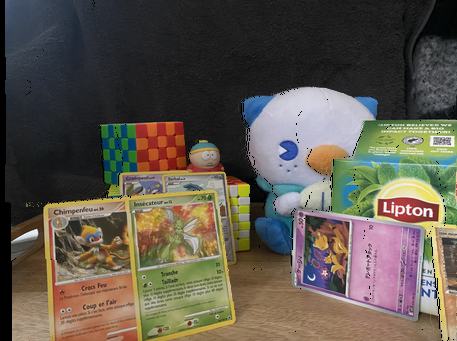
\includegraphics[width=0.95\textwidth]{assets/viewsynthesis/image_11_forwards}
    \end{minipage}%
    \hfill
    \begin{minipage}{.5\textwidth}
        \centering
    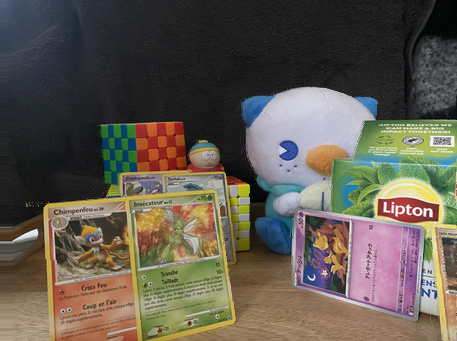
\includegraphics[width=0.95\textwidth]{assets/viewsynthesis/image_11_backwards}
    \end{minipage}
    \caption{The synthesized view point using forwards (left) and backwards (right) view synthesis.}
    \label{fig:vs_forward_backward}
\end{figure}

Performing view synthesis to generate a certain number of viewpoints between the two reference images is easy, and all
that is left to do is to build a quilt and project it on a lenticular display.
We generate a quilt of size $11\times 6$ and thus synthesize $66$ images.
Experimentally, we found that only varying $\alpha$ uniformly between 0 and 1 did not yield a large enough parallax
effect.
Hence, we decided to create 66 images for a varying $\alpha$ between $-0.6$ and $1.6$.
The images generated for values of $\alpha$ outside the regular range ($[0,1]$) are necessarily of lesser quality than
the others because they correspond to viewpoints ever more to the left than the left input image (or to the right
than the right input image), but it does not really matter on small screens and the effect is still quite convincing.

We observe that there are small artifacts in the output views, which we believe are caused by rescaling artifacts in
the disparity maps (the images were too big to be processed and had to be scaled down) as well as the manual cleanup
(which was done by mostly eyeballing both the edges of objects and the disparity).

The full source code associated to this section, as well as the generated images, the generated quilt and a video
of the lenticular display are provided alongisde this report (\textit{QV.2}).

PSNR is a measure of the quality of a reconstructed image.
We have taken a picture of the scene at the halfway point between the left and right images.
This gives a reference image $R$.
For a generated image $I$, the PSNR for a component $c$ (like a specific color channel) is computed as follows,
for a bit depth $b$:
\begin{gather*}
    \text{MSE}_c=\frac{1}{mn}\sum_{i=1}^{n} \sum_{j=1}^{m} [R(i,j)_c-I(i,j)_c]^2\\
    \text{PSNR}_c=10\log_{10}\left(\frac{(2^b-1)^2}{\text{MSE}_c}\right)
\end{gather*}
On the pair of images of figure~\ref{fig:vs_output}, we find a PSNR value of $20.25 dB$, which is relatively poor.
This is easily explained by the fact that the two images slightly differ in camera position (it is clear when
superposing the two images and alternating between them).

\begin{figure}[ht]
    \centering
    \captionsetup{justification=centering}
    \begin{minipage}{.5\textwidth}
        \centering
    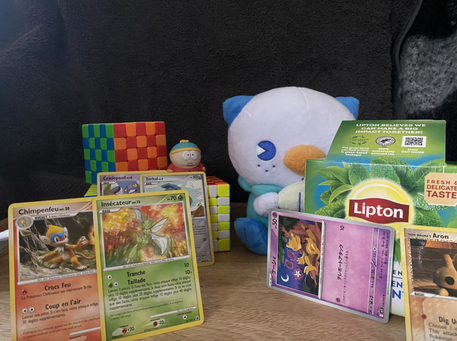
\includegraphics[width=0.95\textwidth]{assets/viewsynthesis/mid_rect}
    \end{minipage}%
    \hfill
    \begin{minipage}{.5\textwidth}
        \centering
    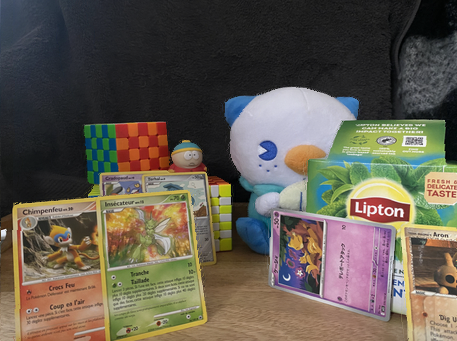
\includegraphics[width=0.95\textwidth]{assets/viewsynthesis/image_30_backward}
    \end{minipage}
    \caption{The true mid-view (left) and the equivalent view generated using backwards view synthesis (right).}
    \label{fig:vs_output}
\end{figure}

IV-PSNR~\citep{ivpsnr} is an equivalent to PSNR but for immersive video (hence the \enquote*{IV} prefix).
The idea is very similar to the regular PSNR except that the corresponding pixel in the generated image $I$ is taken to
be the best candidate in a square window of radius $B$, instead of having to be exactly $(i,j)$:
\[\text{IV-MSE}_c=\frac{1}{mn}\sum_{i=1}^{n} \sum_{j=1}^{m} \min_{\substack{i-B\leq i'\leq i+B\\j-B\leq j'\leq j+B}}
[R(i,j)_c-I(i',j')_c+\text{GCD}_c]^2\]
Where $B$ is the width of a window and $\text{GCD}_c$ is the average global component difference:
\[\text{GCD}=\frac{1}{mn}\sum_{i=1}^{n} \sum_{j=1}^{m}[R(i,j)_c-I(i,j)_c]\]
This gives a more way of computing the PSNR for videos or for synthesized images with slight pixel translations that
are usually not noticeable.
As a sidenote, the IV-PSNR is not symmetric as-is ($R$ and $I$ are not interchangeable and
to make it symmetric, it could be evaluated as the minimum of the IV-PSNR in both directions).

The authors of~\citep{ivpsnr} have provided a tool that can be used to compute the IV-PSNR easily, available
at~\url{https://github.com/jstankowski/ivpsnr}.
This tool computes both the PSNR and the IV-PSNR (as well as the WS-PSNR and the IV-SSIM).
The computed value for the IV-PSNR is $32.08 dB$, which is good (\textit{QV.3}).